\section{Results}
\label{sec:results}

\begin{table}[t]
\centering
\small
\begin{tabular}{lr}
\toprule
Train queries & 1211 \\
\quad with an explicit year (rule extractor) & 43.4\% \\
\quad with a relative time expression & 65.6\% \\
\quad marked temporal in the guidance & 95.0\% \\
Gold documents per query & 3.60 \\
\midrule
Corpus documents with $\geq$1 year & 39.7\% \\
Gold documents with $\geq$1 year & 53.4\% \\
BM25 top-10 non-gold with $\geq$1 year & 65.4\% \\
\midrule
\multicolumn{2}{l}{\textit{Queries with an explicit year:}} \\
\quad gold docs overlapping a query year & 34.0\% \\
\quad BM25 top-10 non-gold overlapping & 42.6\% \\
\bottomrule
\end{tabular}
\caption{Temporal statistics of RETECO Track~1 (train). Gold evidence carries \emph{fewer} explicit years, and overlaps the query's years \emph{less} often, than the non-relevant documents BM25 ranks highly.}
\label{tab:data}
\end{table}
\begin{table}[t]
\centering
\small
\begin{tabular}{lcccc}
\toprule
 & \multicolumn{2}{c}{\textbf{1a}} & \multicolumn{2}{c}{\textbf{1b}} \\
\cmidrule(lr){2-3}\cmidrule(lr){4-5}
\textbf{System} & train & dev & train & dev \\
\midrule
BM25 (official) & .108 & .115 & .102 & .118 \\
BM25 passages + MaxP & .180 & .197 & .191 & .223 \\
Dense (Qwen3-Emb.-0.6B) & .231 & .297 & .246 & .314 \\
Hybrid pool (train-selected) & .273 & .332 & .305 & .325 \\
\sys (final) & .302 & .371 & .310 & .341 \\
\bottomrule
\end{tabular}
\caption{Macro nDCG@10 on RETECO Track~1 (v1.1).}
\label{tab:main}
\end{table}

Table~\ref{tab:main} gives the headline numbers; Table~\ref{tab:full} in
Appendix~\ref{app:full} lists every system with recall@100 and significance against our
passage-level BM25.

\paragraph{Passages explain most of the baseline gap.} Scoring 200-word passages with MaxP
instead of whole documents raises BM25 from \rOfficialA{} to \rBmA{} (1a) and from
\rOfficialB{} to \rBmB{} (1b) with the same $k_1$ and $b$. TEMPO documents include long dumps
whose length normalisation buries the one relevant paragraph; the gain is largest where the
official scores are near zero (\emph{bitcoin}, \emph{monero}, \emph{quant}, \emph{workplace};
Figure~\ref{fig:domains}).

\paragraph{Date matching does not help.} Every temporal device built on explicit years is
neutral or harmful when added to BM25: the prior's weight selected on train is (near) zero
(\rPriorExpA{} vs.\ \rBmA{}), temporal PRF does not change this (\rPriorTprfA{}), fusing the
year-index-filtered run costs \rBmA{}$\rightarrow$\rBmTimeA{}, and the temporal KG costs
\rBmA{}$\rightarrow$\rBmKgA{}. Down-weighting year tokens in the query is also slightly
harmful (\rBmYhalfA{}, \rBmYzeroA{}), so dates are useful query terms, but already exploited by
BM25. Table~\ref{tab:data} explains why: gold documents mention years \emph{less} often than
the non-relevant documents BM25 retrieves, and overlap the query's years less often
(\pctGoldOverlap{} vs.\ \pctTopOverlap{}). RM3 also hurts (\rRmA{}): feedback documents of
long StackExchange questions are noisy.

\paragraph{Dense retrieval is the strongest single channel.} Qwen3-Embedding-0.6B over
passages reaches \rDenseA{} (1a) and \rDenseB{} (1b), and its document-vector variant
\rDenseDocA{} (1a). Equal-weight fusion with BM25 is \emph{below} dense alone
(\rBmDenseA{}), which is why the pool is selected with weights on train.

\paragraph{Temporal RAPTOR.} The collapsed tree performs on par with flat dense retrieval
(\rRaptorA{}/\rRaptorTA{} for the plain/temporal tree on 1a, \rRaptorB{}/\rRaptorTB{} on 1b):
cluster smoothing and child expansion neither help nor hurt much when the leaves are already
strong, and adding the time dimension to the clustering changes little on its own. Its
value is complementarity: forward selection adds the temporal tree to the 1b pool, where its
cluster-expanded candidates raise recall beyond flat dense retrieval. Unlike LLM-summarised
RAPTOR, our centroid tree adds no new text to match against; we return to this in the
limitations.

\paragraph{LLM query planning.} Every LLM-derived channel beats BM25 on 1a:
query2doc reaches \rQtdA{}, keyword expansion \rKwA{} and multi-query with the event chain
\rMultiA{}, against \rBmA{}. Conditioning the planner on the top BM25 snippets (LLM-PRF) helps
consistently on train and gives the best 1a channels on dev (\rQtdFbA{} and \rMultiFbA{}),
while statistical feedback (RM3, \rRmA{}) hurts: the LLM keeps the vocabulary of the feedback
documents that fits the question and discards the rest. On 1b the gains shrink (\rMultiFbB{}
for LLM-PRF multi-query vs.\ \rBmB{}), since plans describe the parent question rather than
the step. The planner agrees with the gold temporal intent for \plannerIntentAcc{} of dev
queries and, when the gold anchors contain a year, its window covers one of them for
\plannerWindowHit{}; it produces \plannerEvents{} events per question on average. Alone, the
LLM channels stay below dense retrieval, but they are complementary to it: forward selection
adds LLM-PRF query2doc to the pool in both sub-tracks (next paragraph).

\paragraph{Hybrid pool.} Forward selection on train picks \poolChannelsA{} for 1a and
\poolChannelsB{} for 1b, reaching \rPoolA{} / \rPoolB{} on dev with recall@100 of
\rRecallPoolA{} / \rRecallPoolB{} (BM25: \rRecallBmA{} / \rRecallBmB{}).

\begin{table}[t]
\centering
\small
\setlength{\tabcolsep}{4pt}
\resizebox{\columnwidth}{!}{%
\begin{tabular}{llcccc}
\toprule
 & & \multicolumn{2}{c}{\textbf{1a dev}} & \multicolumn{2}{c}{\textbf{1b dev}} \\
\cmidrule(lr){3-4}\cmidrule(lr){5-6}
\textbf{Reranker} & & pure & $\oplus$pool & pure & $\oplus$pool \\
\midrule
none (BM25 $\oplus$ dense) & & \multicolumn{2}{c}{.281} & \multicolumn{2}{c}{.309} \\
MiniLM-L12 (33M) & enc. & .179$^{\dagger}$ & .258$^{\dagger}$ & .233$^{\dagger}$ & .296$^{\dagger}$ \\
BGE-v2-m3 (568M) & enc. & .215 & .277$^{\dagger}$ & .275$^{\dagger}$ & .317$^{\dagger}$ \\
Qwen3-Rerank. 0.6B & dec. & .283$^{\dagger}$ & .320$^{\dagger}$ & .319$^{\dagger}$ & .341$^{\dagger}$ \\
Qwen3-Rerank. 4B & dec. & .352$^{\dagger}$ & .352$^{\dagger}$ & -- & -- \\
\bottomrule
\end{tabular}}
\caption{Pointwise reranking of the same top-100 (BM25 $\oplus$ dense, RRF): encoder cross-encoders vs.\ decoder LLM rerankers (``cross-decoders''). \emph{pure}: sorted by the reranker; $\oplus$\emph{pool}: RRF of reranker and pool ranks. Macro nDCG@10, dev.}
\label{tab:rerank}
\end{table}

\paragraph{Cross-encoders vs.\ cross-decoders.} Table~\ref{tab:rerank} compares four rerankers
on the same top-100 (BM25 $\oplus$ dense, \rBmDenseA{} on 1a). The two encoder cross-encoders
\emph{hurt} when used alone (MiniLM \rMiniLMA{}, BGE-v2-m3 \rBgeA{}) and only approach the
candidate ranking when fused with it: trained on short web passages, they reward lexical
overlap with long StackExchange questions. The decoder rerankers, prompted with RETECO's
notion of relevance, improve on it: Qwen3-Reranker-0.6B reaches \rQsmallRRA{} alone and
\rQsmallRRPoolA{} fused, and the 4B model \rQbigRRA{} (\rQbigRRPoolA{} fused). On 1b the
picture is the same (\rMiniLMB{}, \rBgeB{} and \rQsmallRRB{} alone vs.\ \rBmDenseB{}). The gap
between the encoder and decoder families is larger than the gap between the two decoder sizes,
so the LLM backbone and the task instruction matter more than scale here.

\paragraph{Final system.} \sys fuses the train-selected pool with the candidates reranked by
the reranker whose fused system is best on train for the sub-track---\finalRerankA{} for 1a and
\finalRerankB{} for 1b (the 4B model is not a 1b candidate, see \S\ref{sec:setup}). It reaches
\rFinalA{} (1a) and \rFinalB{} (1b) nDCG@10 on dev with recall@100 of \rRecallFinalA{} /
\rRecallFinalB{}: \gainOfficialA\% / \gainOfficialB\% above the official baseline and
\gainBmA\% / \gainBmB\% above our passage BM25 (paired randomisation test against dense
retrieval: $p\,$\pFinalDenseA{} / $p\,$\pFinalDenseB{}). On train~1b the BGE and Qwen3-0.6B
fusions are tied (.310 vs.\ .309); on dev the latter would reach \rLateQsmallB{}, so the 1b
choice is conservative. All final-fusion variants are listed in Table~\ref{tab:full} (Appendix~\ref{app:full}).

\begin{figure}[t]
  \centering
  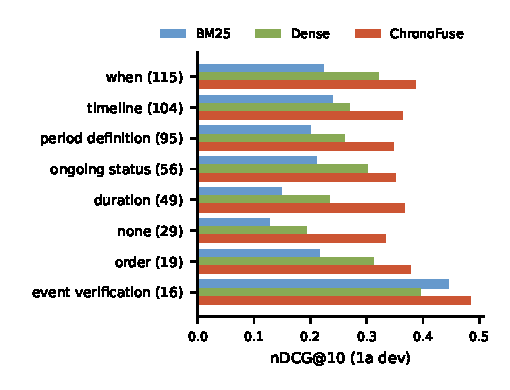
\includegraphics[width=\columnwidth]{figures/intent.pdf}
  \caption{nDCG@10 by gold temporal intent (1a dev; guidance used for analysis only).
  Number of queries in parentheses.}
  \label{fig:intent}
\end{figure}

\begin{figure*}[t]
  \centering
  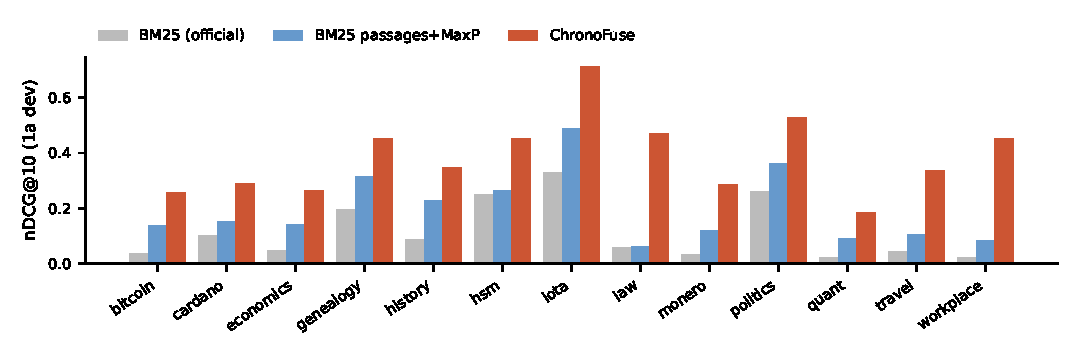
\includegraphics[width=0.9\textwidth]{figures/per_domain.pdf}
  \caption{Per-domain nDCG@10 on 1a dev: official document-level BM25, our passage BM25, and
  \sys.}
  \label{fig:domains}
\end{figure*}

\paragraph{Per-domain and per-intent analysis.} \sys improves over the official baseline and
over passage BM25 in every domain (Figure~\ref{fig:domains}); the largest absolute gains are on
\emph{law}, \emph{workplace} and \emph{iota} ($+$.23 to $+$.36 nDCG@10). By gold temporal intent (Figure~\ref{fig:intent}), the largest
gains over BM25 are for \emph{duration} (.149$\rightarrow$.361) and non-temporal questions
(.128$\rightarrow$.312), whose evidence rarely repeats the question's wording, followed by
\emph{when} and \emph{period definition}. The only intent where BM25 is competitive is
\emph{event verification} (16 questions), where the question names the event to be checked and
lexical matching already finds it.
